\clearpage
\newpage
\section{SafeDE concept}

This section presents the architecture of SafeDE, its features and limitations, its extension towards N-modular redundancy, and its implementation and integration (both hardware and software) details.

SafeDE VHDL files along with its bare metal driver and documentation, are uploaded to a GitLab public repository under a MIT License \cite{SafeDEgit}.

\subsection{Architecture}

SafeDE is built on the light-weight lockstepping concept. As explained in the section \ref{section:software_light_lockstep}, this approach has already been implemented in software. However, the implemented software light-weight lockstep needs a third core running the monitor thread and the frequency at which the monitor can retrieve the executed instruction, compute the staggering and apply corrective measures is low. As a consequence, the long feedback loop imposes a large staggering. 

SafeDE is a tiny hardware module that monitors the execution of the redundant cores imposing some staggering to reach time diversity. As shown in Figure \ref{fig:SafeDE_Arch} SafeDE collects every cycle the instructions executed by the two cores ($\#instr_{head}$ and $\#instr_{trail}$) and computes the staggering that exists between both cores ($instr_{head} - instr_{trail}$). If the head core is not at least $TH_{stag}$ instructions ahead of the trail core ($instr_{head} - instr_{trail} < TH_{stag}$), SafeDE will raise the trail core stall signal that freezes its pipeline registers (registers keep the same value). The stall signal will be set to zero whenever the head core makes enough progress and the staggering is again bigger than $TH_{stag}$ instructions.

$TH_{stag}$ is the minimum staggering (in terms of instructions number) that SafeDE enforces between both cores. Typically, $TH_{stag}$ has a low value. For instance, a value bigger than the pipeline stages can be selected to ensure that the content of both pipelines is always completely different. Hence, the staggering enforced by SafeDE is much smaller than that enforced by the software approach, and it is comparable to the hardware-based lockstep execution staggering. Since SafeDE is implemented directly on hardware is capable of computing the staggering and stalling any of the cores every cycle, overcoming the light-weight lockstepping limitations while maintaining its advantages.

As in the light-weight software-based lockstep execution, a software mechanism must be implemented to compare the results of the executions once they finish. 

Note that the execution of the redundant critical tasks has to be independent. Each critical task has to be allocated in a different memory space address for that purpose. SafeDE is controlled by means of internal registers. Each core has to configure SafeDE once it reaches the critical section that needs lockstepped execution. SafeDE configuration is performed using the corresponding driver. An API is also needed to schedule both redundant processes to the corresponding cores. Later in section \ref{section:software_integration} these software components are described both in the context of bare metal and Linux integrations.

Note that neither core has a pre-defined head or trail core role. The first core indicating SafeDE that has reached the section needing lockstepped execution (i.e., the critical section) assumes the head core roll while the other core assumes the trail roll.

\begin{figure}[h]
    \centering
    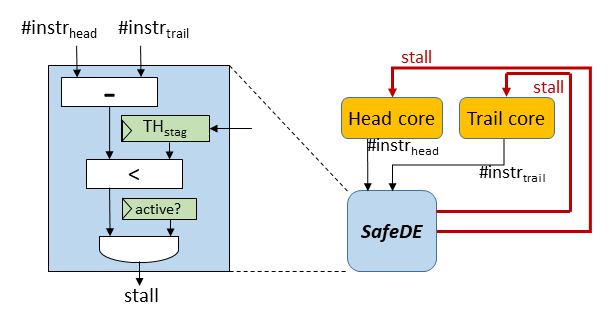
\includegraphics[scale=1]{img/SafeDE_HW.png}
    \caption{SafeDE architecture}
    \label{fig:SafeDE_Arch}
\end{figure}

\bigskip



\subsection{Features and limitations analysis}
\label{section:SafeDE_limitations}

In this section, the main SafeDE limitations and features are presented and compared against the limitations and features of the software-only approach.

\bigskip

\textbf{SafeDE features:}

\begin{itemize}
    \item \textbf{Low cost:} The light-weight software-based lockstep approach needs a third monitor to run the monitor thread. On the contrary, SafeDE is a tiny hardware module that monitors the execution preventing the system from needing a third core. SafeDE implementation requires few resources. In a SoC that integrates four RISC-V cores, SafeDE employs less than 0.5\% of the FPGA resources of the SoC. A more detailed view of the FPGA resources employed by SafeDE is shown in the section \ref{section:Hardware_resources}.

    \item \textbf{Low staggering:} SafeDE checks the executed instructions by both cores every cycle and computes the staggering. Such short feedback allows SafeDE to impose very small staggering (e.g., few instructions 10-20). On the contrary, as discussed, the software-only solution needs staggering values of many thousands of instructions.

    \item \textbf{Flexibility:} SafeDE can be easily enabled and disabled at will and almost immediately. Hence, the limitation is rather imposed by the creation of the redundant software processes, which requires much more time than SafeDE initialization. 

    \item \textbf{Low intrusiveness:} SafeDE needs a few signals from the core's internal pipeline. First, it needs a signal that indicates SafeDE when a new instruction has been committed. Second, it needs a signal that provides a mechanism to stall the core's pipeline when the signal rises. These modifications are much smaller than those that a tight lockstep implementation would require. The software-only implementation does not require hardware modification, but, unlike SafeDE, it may require modification in the operating system to allow the monitor thread to read the instruction count of the redundant cores. 
\end{itemize}

\bigskip

\textbf{SafeDE limitations:}

\begin{itemize}
    \item \textbf{Non-null intrusiveness:} Even though the hardware modifications required by SafeDE are light, they are not null, and unlike the software-only solution, SafeDE can not be built with COTS products.

    \item \textbf{Limited applicability:} Light-weight lockstepping (either software or hardware)  assumes that both redundant executions follow identical instruction streams. Both the hardware and software-only approaches rely on the count of the executed instructions. If the execution paths diverge, a different number of executed instructions will not prevent both cores from exposing the same internal state. This limitation restricts the light-weight lockstepping approach to programs whose control path is deterministic. Thus, SafeDE is unsuitable for applications that make decisions based on random variables and parallel programs that could differ in the number of executed instructions due to the synchronization primitives. Also, programs performing I/O operations would perform these I/O operations twice at different time instants. These could affect the functionality of the system or two different values could be read, causing different results between redundant executions. Note that these limitations apply to light-weight lockstepping.

    \item \textbf{Limited diversity:} SafeDE creates time diversity between two redundant cores forcing a staggered execution. However, even though SafeDE protects the system against some key CCFs, those CCFs whose coupling channel is related to the hardware design or fabrication process (e.g., identical physically weak gates in both cores) will represent a hazard for the system. To protect the system against these CCFs, other types of diversity such as layout diversity must be applied. As mentioned in the section \ref{section:CCFs}, this kind of diversity only can be reached by different hardware designs or by applying different designs at any of the abstraction layers of the ASIC design.

    \item \textbf{SafeDE hardening:} SafeDE is also susceptible to single faults. For instance, a transient fault could affect SafeDE in such a way that the fault propagates to the output leading SafeDE to a failure. In this situation, both cores could reach the same internal state becoming vulnerable in the event of a CCFs. For this reason, the tight lockstep scheme shown in Figure \ref{fig:HWlockstep} must be replicated but substituting the cores with SafeDE modules. 
\end{itemize}


\bigskip

\textbf{Scope of applicability:}

As mentioned, light-weight lockstepping (either hardware or software) has limited applicability (e.g., same instructions streams or no I/O operations). Therefore, two redundant cores coupled with SafeDE can be employed to execute critical code regions rather than entire programs. For instance, in a multicore system implementing eight cores, two must implement tight hardware-based locksteppping to handle the I/O operations while the rest can be coupled with SafeDE. With this configuration, the system can execute several combinations of lockstepped and non-lockstepped tasks, varying from 4 critical tasks to 1 critical task and 6 non-critical tasks. Therefore, the user sees 7 cores instead of 4 cores that would see if all the cores were coupled with a tight lockstepping mechanism. Hence, the performance is almost double using light-weight hardware-based lockstepping approach.

\bigskip




\subsection{N-modular redundancy}

We have developed, implemented and assessed SafeDE in the context of dual-modular redundancy (DMR). However, the SafeDE concept can be easily extended to N-modular redundancy. Some domains (e.g., avionics or medical) could require a safety level that is only achieved through 3-modular redundancy or even 5-modular redundancy. 

In order to extend SafeDE functionality to a system needing N-modular redundancy $N-1$ SafeDE modules are required. For instance, in the case of triple-modular redundancy (TMR), two SafeDE modules would couple $core_1$ and $core_2$ ($SafeDE_{1-2}$) and $core_2$ and $core_3$ (SafeDE 2-3). In this scenario, assuming we want $core_1$ to be ahead in the execution, $core_1$ must be the first one indicating $SafeDE_1$ that it has reached the critical section, becoming the head core. $Core_2$ would be the second one entering the critical section, becoming the trail core w.r.t $core_1$, and the head core w.r.t the $core_3$. Finally, $core_3$ would enter the critical section the last, becoming the trail core w.r.t the $core_2$. This scheme can be extended for N-modular redundancy, where each $core_i$ will always exhibit a staggering  bigger than $TH_{stagg}$ w.r.t the $core_{i+1}$. Unlike DMR, in N-modular redundancy provided $N>2$, the order in which redundant cores access the critical section must be controlled.  

Figure \ref{fig:N_modular_redundancy} shows the concept of flexible N-modular redundancy in a 8-core multicore setup. Seven ($N-1$) SafeDE modules are developed to pair all the consecutive cores in the system. By activating the appropriate SafeDE modules, we can obtain any possible combination of N-modular redundancy. For instance, in the system depicted in Figure \ref{fig:N_modular_redundancy}, TMR is implemented in the cores 1-3 while two core couples (4-5 and 7-8) exibit DMR. Finally, $core_6$ runs independently. This particular configuration is achieved by activating a given subset of the implemented SafeDE modules. In Figure \ref{fig:N_modular_redundancy} activated SafeDE modules are the blue-colored ones, while the inactive ones are the black-colored.


\begin{figure}[h]
    \centering
    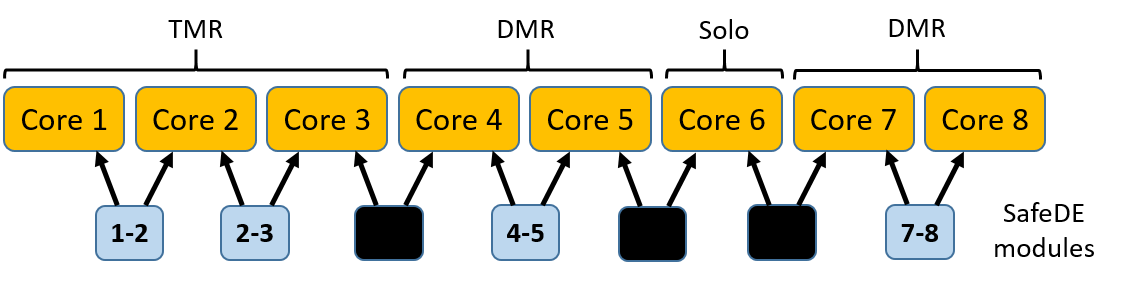
\includegraphics[scale=0.75]{img/Nmodular.png}
    \caption{N-modular redundancy scheme example with SafeDE}
    \label{fig:N_modular_redundancy}
\end{figure}

\bigskip



\subsection{SafeDE Implementantion and Integration}

We have integrated SafeDE in two different multiprocessor platforms based on CAES Gaisler RISC-V NOEL-V cores. This section describes both platforms and provides detailed information on the SafeDE hardware implementation and integration. Later, the SafeDE configuration process is explained. Finally, SafeDE software integration is reviewed both for a bare metal setup and for a platform running Linux.    


\subsubsection{De-RISC and SELENE Platforms}

\textbf{De-RISC platform:} The De-RISC platform \cite{gomez2020risc} is developed in the scope of a European project motivated by the lack of a high-performance Multiprocessor System on a chip (MSPSoC) suitable for space applications. Most of the existing platforms do not supply the necessary performance required by spacecraft, are not reliable enough and are not compliant with the safety requirements for space applications or face export restrictions like the use of proprietary Instruction Set Architecture (ISA). 

The project tries to overcome these limitations by adopting multicore processors in the space domain that provide the required performance but face some challenges related to space safety regulations, predictability and reliability. To avoid export restrictions due to proprietary ISAs, the platform is based on the open-source RISC-V ISA. 

De-RISC platform is composed of different reusable IP cores developed by CAES Gaisler. Those IP cores are contained in the GRLIB IP library, an integrated set of reusable IP cores designed for SoC development. The IP cores have a common on-chip bus interface. SafeDE has been added to the GRLIB IP library as another reusable IP core. The library includes cores for AMBA AHB/APB control. The library is provided under the GNU GPL license.

As a proof of concept, we have integrated SafeDE into the De-RISC industrial space platform. The platform is configured to instantiate 2 CAES Gaisler's NOEL-V 64-bit cores. NOEL-V cores implement the RISC-V ISA, are dual-issue, and implement a 7-stages pipeline. Both cores have one private L1 data and instructions caches. The IP cores are centered around several AMBA AHB and APB buses. Cores are connected to the L2 cache and some peripherals through a 128-bit AMBA Advanced High-performance Bus (AHB). A 32-bit low-bandwidth Advanced Peripheral Bus (APB) is instantiated for components requiring low bandwidth and is connected to the main AHB Bus through an AHB/APB bridge. The L2 cache is shared for all the cores and is connected to the Memory controller through another 128-bit AHB bus.


\textbf{SELENE platform:} SELENE \cite{SELENEgit} is another European project that focuses on developing a High-Performance Computing (HPC) Multicore platform capable of delivering the computation capabilities needed by autonomous systems in safety-critical domains such as space, avionics, robotics and factory automation. HPC platforms impose some difficulties when being certified for safety-critical systems since they usually lack support for functional and timing isolation and testability. The project tries to overcome these limitations by developing an open-source Safety-critical Cognitive Computing Platform (CCP) with self-awareness, self-adapting, and autonomous capabilities. 

SELENE computing platform builds upon a combination of multicore and accelerators that will be prototyped on an FPGA so that they can be extended and upgraded. SELENE platform is also developed using the IP CORES from GRLIB IP CAES Gaisler and other GPL IP cores developed by other project partners. SafeDE is one of the IP cores devised to be integrated into the SELENE platform to make it safer.

SELENE platform is very similar to the De-RISC platform since the basic IP cores used to build the platform are implemented from the GRLIB IP library. However, the SELENE platform offers more complexity since it instantiates more NOEL-V cores and shared L2 cache interconnects with a Network on a Chip, including several Artificial Intelligence (AI) accelerators.

The results and conclusions of this work come from the experiments performed on the De-RISC platform. However, SafeDE is not integrated into the official version of the De-RISC project and the integration was made only as a research exercise. Regarding the SELENE project, SafeDE is one of the safety IP cores integrated into the platform's final version to cover its safety needs.

\subsubsection{Hardware Implementation and Integration}

Since the system only needs to interface with SafeDE to configure it by modifying its internal registers, it demands low bandwidth. Hence, to avoid unnecessary complexity is connected to the system through an APB interface. As shown in Figure \ref{fig:SafeDE_hardware}, SafeDE is built in three hardware layers developed in VHDL. 

\begin{figure}[h]
    \centering
    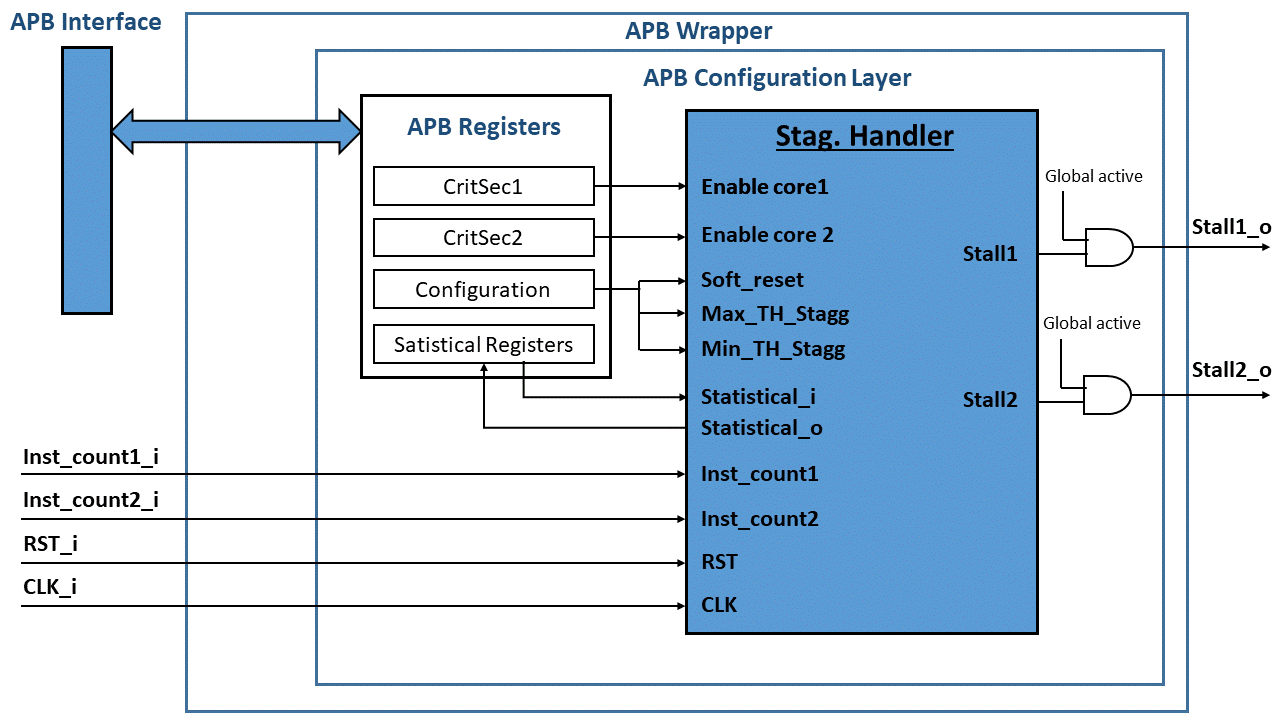
\includegraphics[scale=0.4]{img/SafeDE_hardware.png}
    \caption{High-level representation of SafeDE's hardware}
    \label{fig:SafeDE_hardware}
\end{figure}

\begin{itemize}
    \item The most inner layer called \textit{Staggering Handler} instantiates SafeDE's core functionality. This layer is responsible for calculating the instructions executed by each core, computing the staggering and asserting the stall signal when needed. This layer is completely portable since it is entirely independent of the platform interface. 
    \item The second layer, the \textit{APB configuration layer}, implements the APB protocol. Configuration and statistical registers are also implemented in this layer. This layer allows the AHB masters (cores) to interface with SafeDE and read and write SafeDE internal registers. The values stored in the internal registers act as inputs for the \textit{Staggering Handler} layer.
    \item Finally, the outer layer is the \textit{APB wrapper} layer. This wrapper converts the defined APB AMBA types from the GRLIB IP library to standard VHDL types. In this way, the first two layers are completely portable for any platform implementing the APB interface.
\end{itemize}

As mentioned, SafeDE needs an internal signal from each core pipeline that provides information about how many instructions each core has executed. SafeDE also needs a signal capable of stalling the cores, stopping their progress whenever the staggering is smaller than the set threshold. 

To provide the information related to the executed instructions, we employed a 2-bit signal \textit{inst\_count}. Each of the bits of the signal provides information about each issue of the core. Whenever the issue commits one instruction, the corresponding bit is set to '1' during one cycle. Each core is modified to feed these signals to SafeDE as inputs. With these signals, SafeDE can compute the executed instructions by both cores from a given time instant. Although the De-RISC and the SELENE platforms implement dual-issue NOEL-V cores, SafeDE can be configured through a generic to work with cores with an arbitrary number of issues. 

Each signal SafeDE uses to stall each of the cores is ANDed with a signal, called holdn, driven in the caches controller. The holdn signal is an active-low signal that freezes the pipeline of the core when it is set to '0', preventing the pipeline registers values from updating. ANDing the holdn and the SafeDE stall signal, the pipeline is held any time one of those signals is set to '0'. For simplicity, SafeDE stall outputs are active-high and their value is inverted later. 

Although it is not among the functionalities for which the SafeDE concept was initially devised, SafeDE also can be configured to set a maximum staggering threshold $Max\_TH_{stag}$. Whenever the staggering between both cores is bigger or equal to the configured threshold ($\#instr_{head} - \#instr_{trail} \geq Max\_TH_{stag}$), the head core is stalled. This is useful to reduce the error detection time when intermediate results of the execution are compared between both cores.

Figure \ref{fig:De-RISC_SafeDE} shows an image of the De-RISC platform with SafeDE controlling the staggering of both cores. As shown in Figure \ref{fig:De-RISC_SafeDE}, SafeDE has 3 32-bit configuration registers (Configuration, CritSec1 and CritSec2) plus several statistic registers to gather execution information.

\begin{figure}[h]
    \centering
    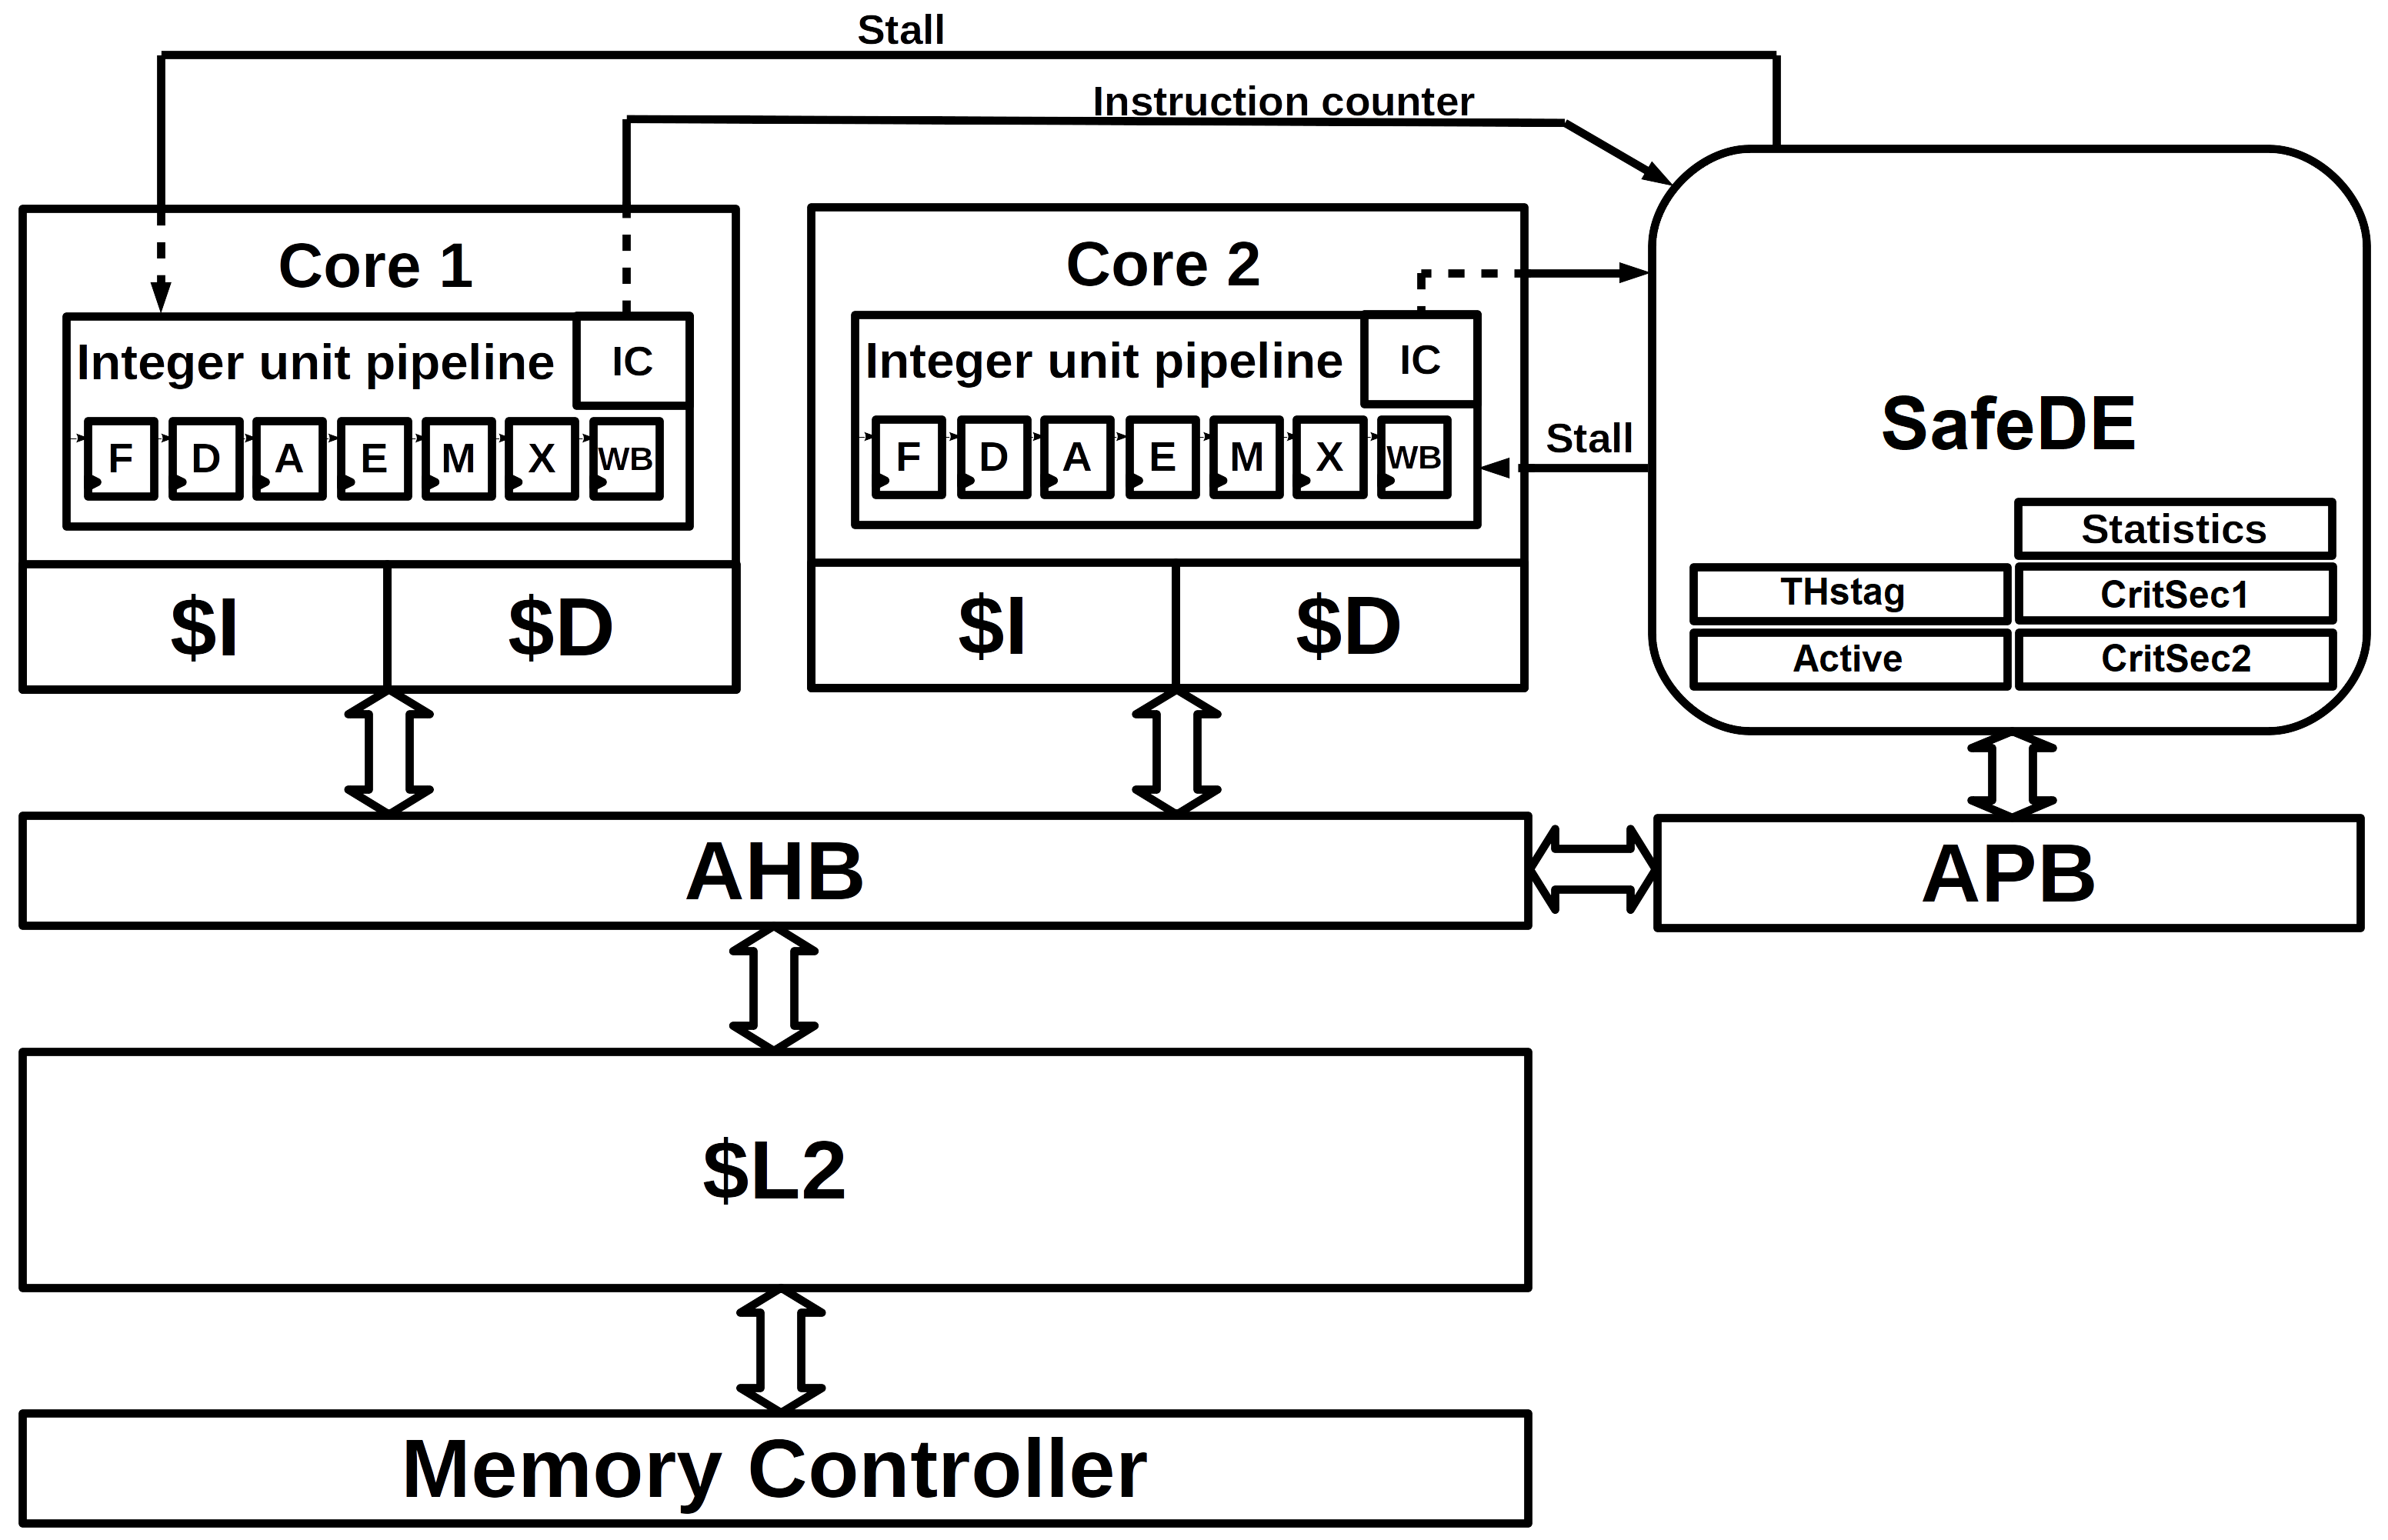
\includegraphics[scale=0.25]{img/system.png}
    \caption{High-level representation of SafeDE integrated into the De-RISC platform}
    \label{fig:De-RISC_SafeDE}
\end{figure}

The bit 31 of the configuration register is used to perform a reset. When this bit is set to '1', SafeDE registers are set to their initial value except for the configuration register. The bit 30 of the configuration register is anded to the output stall signals. Thus, SafeDE is totally neutral and incapable of performing any action over the pipeline if this bit is not set to '1'. The rest 30 bits are used to configure maximum and minimum thresholds for the staggering (15 bits each). Whenever the staggering is bigger or equal to the maximum threshold or smaller or equal than the minimum threshold, the head or trail core will be stalled to keep the staggering within the established limits.  

The first bit of the register CritSec1 must be set to '1' when the core 1 enters the code region needing lockstepped execution. From the moment this bit is set to '1', SafeDE will start counting the instruction executed by core 1. Analogously, core 2 will set the first bit of the register CritSec2. The count of executed instructions will be reset for both cores once the first bit of both CritSec registers is set to '0'. Instead of using two bits of the same register, two different registers (one for each core) are implemented to indicate SafeDE the beginning of the region needing protection. The reason is that two different registers prevent writes from different cores from overriding the other core's bit.

SafeDE statistic registers gather information from the execution. Namely, they collect the following information: Total number of cycles SafeDE has been active, number of executed instructions by each core, number of times each core has been stalled during the execution, number of cycles each core has been stalled during the execution and maximum, minimum and average staggering during the execution.





\subsubsection{Configuration and Operation}

When using SafeDE, the first step is configuring the desired staggering thresholds $Max\_TH_{stag}$ and $Min\_TH_{stag}$. If the $Max\_TH_{stag}$ is not configured, $Max\_TH_{stag}$ will be internally set close to its maximum possible value (32750). After configuring the staggering thresholds, the next step is to set to '1' the activation bit (bit 32 of the configuration register), which is Ored with the stall signals. The first core reaching the code section that needs lockstep protection will set its CritSec register first bit to '1'. From that moment, this core will assume the head roll and SafeDE will start counting each committed instruction. Later, the second core will reach the code region needing protection and set its CritSec register assuming the trail roll. Once one core have set it CritSec register, SafeDE will check that the staggering is within the limits ($Min\_TH_{stag} < \#intst_{head} - \#inst_{trail} < Max\_TH_{stag}$) and will stall any of the cores if needed until the previous condition is met.  

Once the head core has finished the execution, it will set its CritSec register bit to '0'. SafeDE will let the trail core finish the execution without intervention. Once the trail core finishes the execution, it will set its CritSec register bit to '0' analogously to the head core. When both CritSec registers' first bits have value '0', SafeDE will set the instruction counts of both cores to 0.
\bigskip


\subsubsection{Software Integration}
\label{section:software_integration}

We developed the software interface to control SafeDE IP. SafeDE can be employed in two different software environments: In a bare metal setup, where there is no restriction to access the hardware registers directly and a simple C library suffices to handle SafeDE. In a setup with an operating system running on top of it. In this scenario, the operating system is responsible for handling and protecting the hardware and direct hardware access is not granted to the user. Hence, a driver running in the kernel space and an API that performs the communication from the user space to the kernel space are required. Since Linux was ported to the SELENE platform as part of the SELENE project, we developed a driver to procure SafeDE an interface with Linux.

\textbf{Bare metal integration:} To interface with SafeDE in the context of a bare metal setup, we created a simple API consisting of a C library that handles internal SafeDE registers accordingly to perform basic configuration actions. The use of the C library allows the user to control SafeDE without knowing its internal hardware details. The API offers the user functions to reset SafeDE, configure the staggering, enable and disable SafeDE, indicate when each of the cores has reached and has finished the critical section that requires lockstepped execution or retrieve and print the statistics gathered during the execution. 

\textbf{Linux integration:} As mentioned, Linux does not grant the user permission to handle the hardware directly. To allow the user to access SafeDE hardware, a driver that executes inside of the kernel space is needed. The code inside the kernel space executes in machine mode having total control of the platform. Hence, the driver can directly access the hardware. However, the user and the kernel spaces are separated, i.e., they are allocated in different and isolated memory segments. For that reason, the user also needs a mechanism to allow communication between both spaces. The communication link between both spaces in Linux is the device file, a special file created in the Linux file system during the driver initialization process. In addition to the driver, we developed an API that performs the communication from the user space to the kernel space by writing into the device file. As in the bare metal API, this API offers the user functions to perform the aforementioned SafeDE control and configuration actions. However, instead of writing SafeDE registers directly, the Linux API writes a 64-bit integer value into the device file. The value of the integer encodes the information about the action the user wants to perform and its arguments. The driver reads the integer value from the device file and decodes the information to determine the physical address that should be read or written. Finally, the driver transforms the physical address into the equivalent virtual address and performs the read or write operation.

As stated in section \ref{section:SafeDE_limitations}, one of SafeDE's limitations is that both cores have to execute the same instruction stream. This is a problem in a preemptive operating system such as Linux. Imagine that a process writes its CritSec register, indicating SafeDE to start counting committed instructions. If that process is preempted, SafeDE will continue counting executed instructions as if they were executed by the preempted process. Hence, in this situation, SafeDE would lose track of the real amount of executed instructions and lose control over the staggering. Even deactivating the CritSec register would be ineffective since this should occur immediately not to alter the executed instruction count. To avoid this situation, some measures must be adopted:

\begin{enumerate}
    \item In Linux, processes have a mask indicating in which subset of the cores can be executed (a.k.a process affinity). When this mask indicates only one core, it is called binding. Our strategy consists of binding the redundant processes to two specific cores and modifying all the other processes (user and kernel processes), so they do not preempt the critical processes.

    \item Even if the process' affinity is modified when critical redundant tasks are launched, new processes created after that moment could preempt the redundant tasks. To avoid this situation, we must queue the redundant tasks into the Linux scheduler's highest priority queue, which is SCHED FIFO queue. To perform this action, we employ the Linux system call sched setscheduler().
\end{enumerate}

Note that the situation would be different if a real-time operating system (RTOS) was used instead of Linux (e.g., fentISS' XtratuM, SYSGO's PikeOS, RTEMS). These operating systems are designed for safety-related systems and offer simpler task scheduling and priority assignment mechanisms. Hence, preemption of redundant tasks could be avoided much more easily. 


\bigskip